% LaTeX template for Lab Reports
% Copyright (C) 2014 Julian Coy

%% CHANGE REPORT TITLE HERE
\newcommand{\reporttitle}{
 Simple Processor
}

%% HEADER/PREAMBLE INFORMATION

% "The font should be 11pt Times New Roman"
\documentclass[11pt]{report}
\usepackage[T1]{fontenc}
\usepackage[utf8]{inputenc}

\usepackage{mathptmx}               

% "The body of the paper should use 1" margins on all sides."
\usepackage[margin=1in]{geometry}

% "Pages must be numbered, starting with 1 on the first page in the body of the report.
% The cover page should not be numbered. 
% Page numbers should be in the bottom-right corner of the page."
\usepackage{fancyhdr}
\pagestyle{fancy}
\fancyhead{}
\fancyfoot{}
\renewcommand{\headrulewidth}{0pt}
\fancyfoot[R]{\thepage}

% Set up customized spacing
\usepackage{setspace}

% Allows for Trademark Symbols
\usepackage{textcomp}

% Remove spacing between items in lists
\usepackage{enumitem}

% Remove extra spacing between titles of sections and subsections
\usepackage{titlesec}
\titlespacing\section{0pt}{10pt}{10pt}
\titlespacing\subsection{0pt}{10pt}{10pt}
\titlespacing\subsubsection{0pt}{0pt plus 4pt minus 2pt}{0pt plus 2pt minus 2pt}

% Setup the specialized chapter section for the Abstract
\titlespacing\chapter{0pt}{0pt plus 4pt minus 2pt}{0pt plus 2pt minus 2pt}
\titleformat{\chapter}[block]{\centering\Huge}{}{}{}{}

% Set up BibTeX integration using IEEE citation format
\usepackage{cite}
\bibliographystyle{ieeetr}
\usepackage{url}

% Set bibliography to have a section header rather than chapter header
\makeatletter
\renewenvironment{thebibliography}[1]
     {\section*{\scshape Works Cited}% <-- this line was changed from \chapter* to \section*
      \@mkboth{\MakeUppercase\bibname}{\MakeUppercase\bibname}%
      \list{\@biblabel{\@arabic\c@enumiv}}%
           {\settowidth\labelwidth{\@biblabel{#1}}%
            \leftmargin\labelwidth
            \advance\leftmargin\labelsep
            \@openbib@code
            \usecounter{enumiv}%
            \let\p@enumiv\@empty
            \renewcommand\theenumiv{\@arabic\c@enumiv}}%
      \sloppy
      \clubpenalty4000
      \@clubpenalty \clubpenalty
      \widowpenalty4000%
      \sfcode`\.\@m}
     {\def\@noitemerr
       {\@latex@warning{Empty `thebibliography' environment}}%
      \endlist}
\makeatother

% Set up math
\usepackage{amsmath}
\usepackage{amsfonts}
\usepackage{amssymb}

% Set up graphics
\usepackage{graphicx}
\usepackage{float}

% Set up tables
\usepackage{tabularx}
\usepackage{booktabs}

% Set up code blocks
% or not...

\usepackage{listings}
\usepackage{color}

\definecolor{dkgreen}{rgb}{0,0.6,0}
\definecolor{gray}{rgb}{0.5,0.5,0.5}
\definecolor{mauve}{rgb}{0.58,0,0.82}

\lstset{frame=tb,
  language=VHDL,
  aboveskip=3mm,
  belowskip=3mm,
  showstringspaces=false,
  columns=flexible,
  basicstyle={\small\ttfamily},
  numbers=none,
  numberstyle=\tiny\color{gray},
  keywordstyle=\color{blue},
  commentstyle=\color{dkgreen},
  stringstyle=\color{mauve},
  breaklines=true,
  breakatwhitespace=true
  tabsize=3
}

%% START OF DOCUMENT

\begin{document}

% "The main body of text should use 1.5 spacing"
\begin{spacing}{1.5}

% Suppress page numbering on first page
\thispagestyle{empty}

\begin{scshape}

% Title
% "The title should be centered and written in approximately 22pt font."
\vspace*{30pt}
{
\Huge
\begin{center}
    \reporttitle
\end{center}
}
\vspace{30pt}

% Team Number
% "The Team number should be centered and written several lines below the title and should use a
% similar size font as the title."
{
\Large
\begin{center}
  Lab Report 5 for ECE327 \\
  Digital Systems Design
\end{center}
}
\vspace{30pt}
% Team Members
% "Directly below the team identifier, team members should be listed alphabetically by last name, one
% per line, in approximately 14pt font. The column of names should be approximately centered on
% the page, but the names within the column should be left justified (so they all start at the same
% horizontal position)."
{
\Large 
\begin{center}
  Submitted by \\
  Julian Coy
\end{center}
}
\vspace{120pt}

{
\Large
\begin{center}
  Undergraduate of Electrical \& Computer Engineering \\
  Clemson University
\end{center}
}
\vspace{30pt}

{
\Large
\begin{center}
  April 28, 2014
\end{center}
}

\end{scshape}

% New page and reset page numbering
\clearpage

%% START EDITS BELOW %%

\vspace{15pt}
  \setcounter{chapter}{1}
  \chapter*{Abstract}
  \label{cha:abstract}
\vspace{72pt}

A system that can perform different operations based on numerical operations considered a processor.  Processors are the basic control units of all computing.  The task of this lab was to implement a simple processor system.  The first part of the lab was to build a processor that contained a full adder that was also capable of subtraction.  Located in the processor were 8 16-bit registers, as well as other registers required by the system (in this lab, two were needed).  The second part of the lab was to create a memory module that would feed the processor instructions by reading them sequentially from a ROM module.  The final portion of the lab was to identify critical paths in the processor circuit and then postulate methods to obtain the maximum viable frequency.

\vspace{4.5in}

\textit{Note: All clocks generated for simulation were built using Morten Zilmers clock gen package \cite{Synth}.}

\thispagestyle{empty} % clear page number
\clearpage
\setcounter{page}{1}

\section*{\scshape Introduction} %(0.5 pages)
\label{cha:introduction}

The purpose of this lab is to simulate a simple 16-bit processor.  A diagram of the system can be seen in Figure \ref{fig:system}.  The full adder/subtracter and multiplexer will operate instantaneously and not need to be operated by a clock.  The code for each module is provided in the code appendices at the end of the report.

\vspace{15px}
\begin{figure}[H]
    \centering
    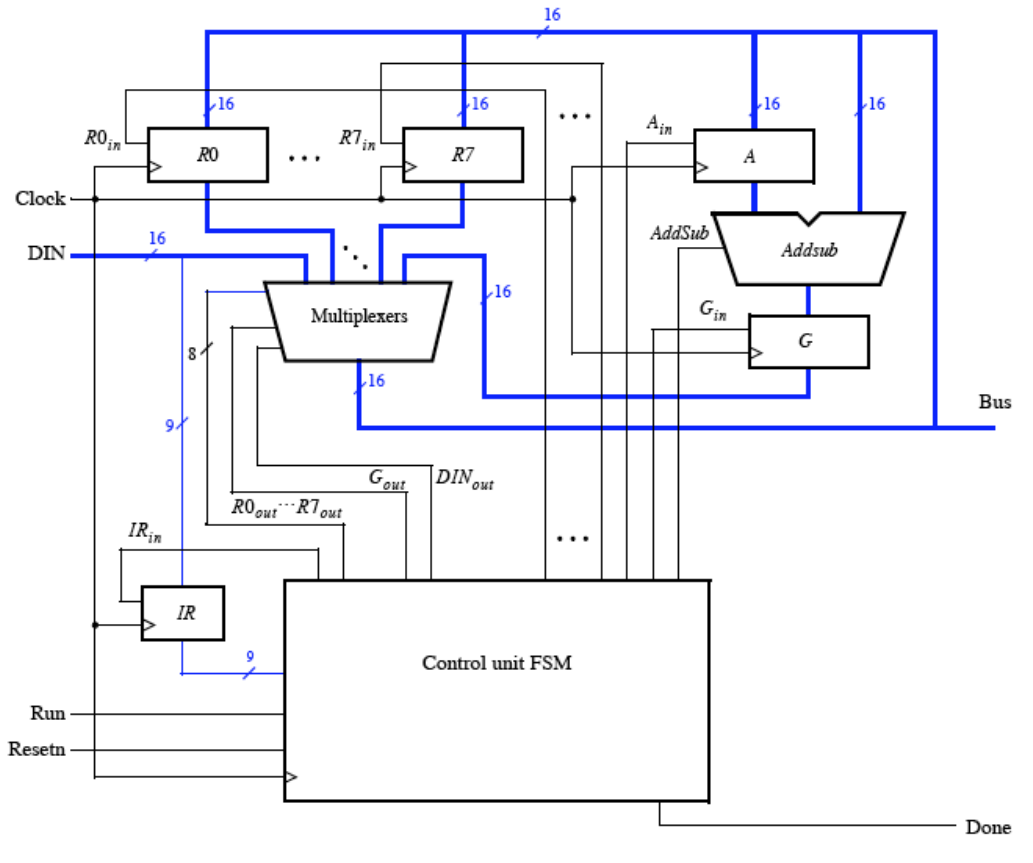
\includegraphics[width=1.0\textwidth,keepaspectratio]{system.png}
    \caption{Simple Processor}
    \label{fig:system}
\end{figure}

There are four main components to this design: the control state module, the registers, the multiplexer, and the full adder/subtracter.  The IR register is similar to the other registers, but only stores a 9 bit value.  The multiplexer logic is contained inside the control FSM due to it's simplicity.

\clearpage

\section*{\scshape Lab 4 System Design - Part I} %(0.5 pages)
\label{sec:fsm_design}

\setcounter{section}{1}
\setcounter{subsection}{0}
\subsection{\scshape Register Design}
\label{sub:design_piso}

There are only two register prototypes in this design, and both are incredibly similar.  Registers 0-7, A, and G are all 16 bit flip flops.  They store a value on the rising edge of the clock only when their select line is driven high.  The instruction register (IR) is the exact same as the others, but only utilizes 9 bit buses and storage.

The only real variation in the registers is their data line connections.  Registers 0-7 feed from a 16 bit data bus and output to the multiplexer.  Register A feeds from the data bus as well, but instead of the multiplexer, it outputs to the full adder/subtracter (adder).  Register G's input is from the output of the adder unit and outputs back into the multiplexer.  The most different of the connections is again for the IR.  The IR captures the 9 MSBs of the data in (DIN) line.  It also outputs its data directly to the control unit.

\subsection{\scshape Testing of the Registers}
\label{sub:test_piso}

Due to the simplicity of the registers, only one unit test was required.  Figure \ref{fig:register} shows the results of the testbench that was run on the register modules.

\vspace{15px}
\begin{figure}[H]
    \centering
    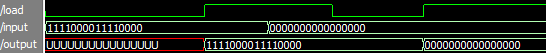
\includegraphics[width=1.0\textwidth,keepaspectratio]{tb_reg.png}
    \caption{Register Loading Results}
    \label{fig:register}
\end{figure}

Notice that on the first rising edge of load, the input is immediately clocked into the output.  The input signal changes during the load pulse, but since there is no rising edge no change occurs.  The new value is then clocked in on the next rising edge.

\setcounter{section}{2}
\setcounter{subsection}{0}
\subsection{\scshape Full Adder/Subtracter Design}
\label{sub:design_piso}

The addition and subtraction module was designed with speed in mind.  In order to achieve this, there would need to be no clock on the adder system.  This means that an instantaneous design based upon gate logic would be optimal.  The appendices show the code used to generate the instantaneous adder/subtracter logic.

\subsection{\scshape Testing of the Full Adder/Subtracter}
\label{sub:test_piso}

Due to the simplicity of the registers, only one unit test was required.  Figure \ref{fig:register} shows the test bench that was run on the register modules.

\vspace{15px}
\begin{figure}[H]
    \centering
    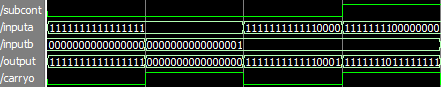
\includegraphics[width=0.8\textwidth,keepaspectratio]{addsubtest.png}
    \caption{Register Loading Results}
    \label{fig:register}
\end{figure}

Notice that on the first rising edge of load, the input is immediately clocked into the output.  The input signal changes during the load pulse, but since there is no rising edge no change occurs.  The new value is then clocked in on the next rising edge.

\setcounter{section}{3}
\setcounter{subsection}{0}
\subsection{\scshape Multiplexer Design}
\label{sub:design_piso}

The multiplexer was created by only one with statement inside the FSM logic.  Due to it's simplicity it will not be discussed in this report.  The code for the multiplexer can be seen on lines 90-100 of lab5.vhd contained in the appendices.

\subsection{\scshape Testing of the Multiplexer}
\label{sub:test_piso}

No testing was required since the multiplexer was implemented as a built-in command in VHDL.

\setcounter{section}{4}
\setcounter{subsection}{0}
\subsection{\scshape Control Unit Design}
\label{sub:design_piso}

The control unit was the most complicated portion of this lab.  The control unit maintained all interconnecting signal lines and program logic across 9 finite states.  Most of the state logic for this lab was sequential, meaning that there were only a few logical branches spread throughout the states.  Due to the linearity of the states, a state diagram was deemed unnecessary.  The only branching occurs in the 4th state, D.  If the branch is accepted the state returns to A, otherwise it continues on in a cyclic cycle.

The reason the processor required 9 states is mainly due to the shared register bus.  This bus required multiple cycles during data transfers, so that data was not improperly sent or duplicated.  It may have been possible to eliminate a few of these states, by creating a more robust multiplexer system that would keep the bus from having collisions.

\subsection{\scshape Testing of the Control Unit}
\label{sub:test_piso}

The control unit testing was fairly simple.  A few commands were sent to the data in line as the clock was cycled.  The key component to this process was making sure the exact amount of clock cycles occurred based upon the data being processed.  This is where the done signal came in handy.  By using the done signal, it was much easier to track when to send new data to the processor.  Figures \ref{fig:fsm} and \ref{fig:fsm2} show the complete testing performed on the FSM logic.

\vspace{15px}
\begin{figure}[H]
    \centering
    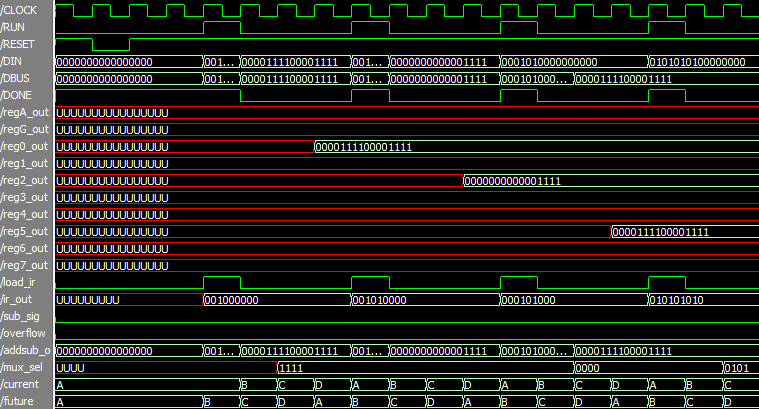
\includegraphics[width=1.0\textwidth,keepaspectratio]{lab5atest.png}
    \caption{FSM Test Part I}
    \label{fig:fsm}
\end{figure}

The test is fairly complicated, so it is easiest to simply examine the register values in the center.  Notice the first instruction loaded is to store 0x0F0F into register 0.  Then 0x000F is stores in register 2.  The third instruction is to copy register 0 to register 5.  Each of these instructions performed flawlessly, but they were all evenly spaced based on data reading.  The next test shows the completion of the addition instruction that is given at the end of Figure \ref{fig:fsm}.

\vspace{15px}
\begin{figure}[H]
    \centering
    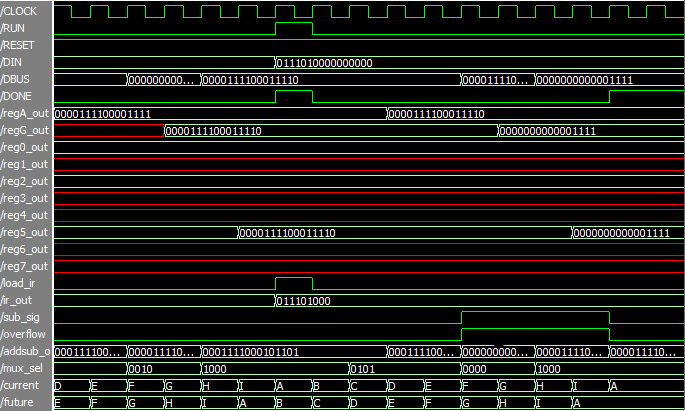
\includegraphics[width=1.0\textwidth,keepaspectratio]{lab5atest_2.png}
    \caption{FSM Test Part I}
    \label{fig:fsm2}
\end{figure}

This test was a continuance of the previous test.  Note that the new value stored into register 5 is the addition of register 5 and register 2.  The final portion of this test bench was to then subtract register 0 from register 5.  This then returns the original value of register 2 which is mathematically correct and verifies the functionality of the FSM logic.

\clearpage

\section*{\scshape Lab 4 Memory Design - Part II} %(0.5 pages)
\label{sec:fsm_design}

\setcounter{chapter}{2}
\setcounter{section}{1}
\setcounter{subsection}{0}
\subsection{\scshape Memory Unit Design}
\label{sub:design_piso}

The memory module was designed by using the Quartus II MegaWizard Plug-In.  There was no coding required to complete the memory module.  A 16 bit wide and 32 word deep read only memory (ROM) module was generated by the wizard.  This system was then incorporated with the processor from part 1 as shown by Figure \ref{fig:memory}.

\vspace{15px}
\begin{figure}[H]
    \centering
    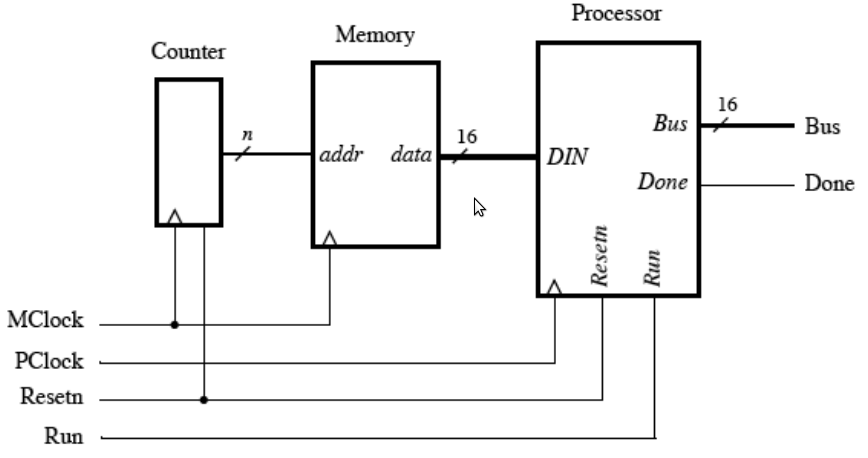
\includegraphics[width=0.75\textwidth,keepaspectratio]{part2.png}
    \caption{Memory and Processor}
    \label{fig:memory}
\end{figure}

\subsection{\scshape Testing of the Memory}
\label{sub:test_piso}

A ROM instantiation file was created, called "inst\_mem.mif".  This file was used to insert instructions into the memory of the ROM.  A testbench was then created that would run memory clock (MClock) long enough to extract instruction data from the memory.   The processor clock (PClock) would continue to run until the Done signal was asserted.  Once the done signal was high, the process would start over with running the MClock to extract the next instruction.  The results from the testbench are shown in Figure \ref{fig:part2}.

\vspace{15px}
\begin{figure}[H]
    \centering
    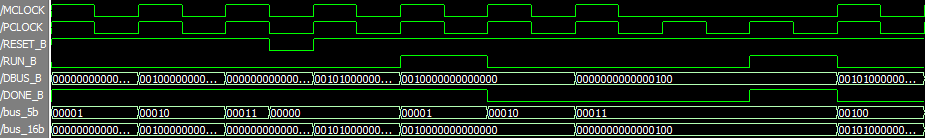
\includegraphics[width=1.0\textwidth,keepaspectratio]{tb_lab5b.png}
    \caption{Memory and Processor}
    \label{fig:part2}
\end{figure}

Note that as soon as the RESET\_B signal goes high, the DBUS\_B displays the instructions from memory in the order that they are coded into the inst\_mem.mif file.  Each time a new instruction is loaded, the counter is increased.  This allows the processor to know which location in memory is currently being executed.  The entire instruction list can be found in Appendix B.

\section*{\scshape Critical Paths and Conclusions - Part III} % (fold)
\label{sec:conclusions}

\setcounter{chapter}{3}
\setcounter{section}{1}
\setcounter{subsection}{0}
\subsection{\scshape Critical Paths}

In order to best modify the processor for real world conditions, we need to identify the critical paths.  By running the TimeQuest analyzer inside the Quartus II software suite, it was abundantly clear that the most critical path in this processor is the jump from state D to A.  This is due to the branching nature of state D.  One possible solution to shortening the path would be to reduce the logic it contains.  This would require minimization of the logic inside the state machine and probably a redesign of the machine using architectural instead of behavioral models.

\subsection{\scshape Conclusions}

In this lab, many components of VHDL and hardware design have come together to build an entire computer.  Although the processor is simplistic in its functioning, adding additional operations would require only fairly simple modifications to the existing structure.  This process is similar to the core concepts of any functioning processor on the market.  Knowledge of this underlying truth is invaluable, and will greatly aid in any computer engineers understanding of computing machines and concepts.

% section scshape_conclusions (end)

\clearpage

% Bibliography

\bibliography{citationsfile}{}


\chapter*{\scshape Appendix A: inst\_mem.mif}
\label{app:a}
\vspace{15px}
\begin{lstlisting}
DEPTH = 32;                   -- The size of data in bits
WIDTH = 16;                    -- The size of memory in words
ADDRESS_RADIX = HEX;          -- The radix for address values
DATA_RADIX = BIN;             -- The radix for data values
CONTENT                       -- start of (address : data pairs)
BEGIN

00 : 0010000000000000;    -- move data into reg0
01 : 0000000000000011;    -- data to move is 0x0003

02 : 0010100000000000;    -- move data into reg2
03 : 0000000000000101;    -- data to move is 0x0005

04 : 0001110000000000;    -- move reg0 to reg7

05 : 0100111100000000;    -- add reg7 to reg2 (3+5=8)

06 : 0010110000000000;    -- move data into reg3
07 : 1111111111111111;    -- data to move is -1

08 : 0011000000000000;    -- move data into reg4
09 : 1111111111111110;    -- data to move is -2

0A : 0001100110000000;    -- move reg3 to reg6

0B : 0001011000000000;    -- move reg4 to reg5

0C : 0100101100000000;    -- add reg6 to reg 2 (8+(-1)=7)

0D : 0110101110000000;    -- subtract reg7 from reg2 (7-3=4)

0E : 0100101010000000;    -- add reg5 to reg2 (4+(-2)=2)

0F : 0110101110000000;    -- subtract reg7 from reg2 (2-3=-1)

10 : 0110101110000000;    -- subtract reg6 from reg2 (-1-(-1)=0)

11 : 0010110000000000;    -- move data into reg3
12 : 0000000000001111;    -- data to move is 0x000F

13 : 0011000000000000;    -- move data into reg4
14 : 0000000011110000;    -- data to move is 0x00F0

15 : 0011110000000000;    -- move data into reg7
16 : 0000111100000000;    -- data to move is 0x0F00

17 : 0011100000000000;    -- move data into reg6
18 : 1111000000000000;    -- data to move is 0xF000

19 : 0010000000000000;    -- move data into reg0
1A : 0000000000001111;    -- data to move is 0x000F

1B : 0010100000000000;    -- move data into reg2
1C : 0000000011111111;    -- data to move is 0x00FF

1D : 0011010000000000;    -- move data into reg5
1E : 1111111100000000;    -- data to move is 0xFF00

1F : 0101010100000000;    -- add reg2 to reg5 0xFF00+0x00FF



END;
\end{lstlisting}

\chapter*{\scshape Appendix A: lab5.vhdb}
\label{app:a}
\vspace{15px}
\begin{lstlisting}
----------------------------
--  Lab 5 FSM Controller  --
----------------------------

library ieee,work;
use ieee.std_logic_1164.all;
USE ieee.numeric_std.all;
use work.all;

entity lab5 is port (
  CLOCK : in std_logic;
  RUN   : in std_logic;
  RESET : in std_logic;
  DIN   : in std_logic_vector(15 downto 0);
  DBUS  : buffer std_logic_vector (15 downto 0) := X"0000"; 
  DONE  : out std_logic := '0');
end entity lab5;

architecture behav of lab5 is
  -- Schignuls
  signal loadreg0 : std_logic;
  signal loadreg1 : std_logic;
  signal loadreg2 : std_logic;
  signal loadreg3 : std_logic;
  signal loadreg4 : std_logic;
  signal loadreg5 : std_logic;
  signal loadreg6 : std_logic;
  signal loadreg7 : std_logic;
  signal loadregA : std_logic;
  signal loadregG : std_logic;
  
  signal loadreg  : std_logic_vector( 9 downto 0);

  signal regA_out : std_logic_vector(15 downto 0);
  signal regG_out : std_logic_vector(15 downto 0);
  signal reg0_out : std_logic_vector(15 downto 0);
  signal reg1_out : std_logic_vector(15 downto 0);
  signal reg2_out : std_logic_vector(15 downto 0);
  signal reg3_out : std_logic_vector(15 downto 0);
  signal reg4_out : std_logic_vector(15 downto 0);
  signal reg5_out : std_logic_vector(15 downto 0);
  signal reg6_out : std_logic_vector(15 downto 0);
  signal reg7_out : std_logic_vector(15 downto 0);

  signal load_ir  : std_logic;
  signal ir_out : std_logic_vector( 8 downto 0);

  signal sub_sig  : std_logic;
  signal overflow : std_logic; -- unused, but part of the adder design
  signal addsub_o : std_logic_vector(15 downto 0);

  signal mux_sel  : std_logic_vector( 3 downto 0);

  -- setup the states and state signals
  type fsm is (A,B,C,D,E,F,G,H,I);
  signal current, future : fsm;

  component reg_16 is
  port( load  : in  std_logic;
      input : in  std_logic_vector(15 downto 0);
      output  : out std_logic_vector(15 downto 0));
  end component reg_16;

  component reg_ir is
  port( load  : in  std_logic;
      input : in  std_logic_vector(15 downto 0);
      output  : out std_logic_vector( 8 downto 0));
  end component reg_ir;

  component addsub_16 is
  port (  subcont : in  std_logic;
      carryo  : out std_logic;
      inputa  : in  std_logic_vector(15 downto 0);
      inputb  : in  std_logic_vector(15 downto 0);
      output  : out std_logic_vector(15 downto 0));
  end component addsub_16;

begin
  -- either continue operation or reset async-ly on active low
  cont_reset : process (RESET, CLOCK)
  begin
    if RESET = '0'
      then current <= A;
    elsif rising_edge(CLOCK)
      then current <= future;
    end if;
  end process cont_reset;

  -- build the mux using simple WITH-SELECT logic
  with mux_sel select DBUS <=
    reg0_out when "0000",
    reg1_out when "0001",
    reg2_out when "0010",
    reg3_out when "0011",
    reg4_out when "0100",
    reg5_out when "0101",
    reg6_out when "0110",
    reg7_out when "0111",
    regG_out when "1000",
    DIN when others;

  fsm_control : process (current, RUN)
  begin
    case current is
    -- oh god, here we go
      when A => -- static state
        if run = '0' then
          future <= A;
          loadreg <= "0000000000"; -- clear all register load lines
          load_ir <= '0';
          sub_sig <= '0';
        else
          future <= B;
          load_ir <= '1';
        end if;
        DONE  <= '1';
      when B => -- load instruction
        DONE  <= '0';
        load_ir <= '0';
        future  <= C;
      when C =>
        case ir_out(8 downto 6) is -- figure out what type of inst
          -- mv, add, or sub
          when "000"|"010"|"011" => -- select YYY from ir, store on bus
            mux_sel(3) <= '0';
            if ir_out(7) = '1' then
              mux_sel(2 downto 0) <= ir_out(5 downto 3);
            else
              mux_sel(2 downto 0) <= ir_out(2 downto 0);
            end if;
          -- mvi
          when others => -- select DIN, store on bus
            mux_sel <= "1111";
        end case;
        future  <= D;
      when D =>
        case ir_out(8 downto 7) is
          -- mv or mvi
          when "00" => -- store bus into register XXX and finish
            loadreg(to_integer(unsigned(ir_out(5 downto 3)))) <= '1'; -- please work
            future <= A;
          -- add or sub
          when others => -- otherwise store DBUS on A and continue
            loadreg(8) <= '1'; -- load regA
            future <= E;
        end case;
      when E => -- clear all flags so we don't double load
        loadreg <= "0000000000";
        future <= F;
      when F => -- since we know we're in a math inst,
        if ir_out(6) = '1' then -- we know were subtracting
          sub_sig <= '1';
        else -- or adding
          sub_sig <= '0';
        end if;
        mux_sel(3) <= '0'; -- now load YYY onto DBUS
        mux_sel(2 downto 0) <= ir_out(2 downto 0);
        future <= G;
      when G => -- store result in G
        loadreg(9) <= '1';
        future <= H;
      when H => -- load G on DBUS
        loadreg(9) <= '0';
        mux_sel <= "1000";
        future <= I;
      when I => -- save DBUS to XXX
        loadreg(to_integer(unsigned(ir_out(5 downto 3)))) <= '1';
        future <= A;
      when others =>
        future <= A;        
    end case;
  end process;

  RegA : reg_16 PORT MAP (
    load  => loadreg(8),
    input => DBUS,
    output  => regA_out
  );

  RegG : reg_16 PORT MAP (
    load  => loadreg(9),
    input => addsub_o,
    output  => regG_out
  );

  Reg0 : reg_16 PORT MAP (
    load  => loadreg(0),
    input => DBUS,
    output  => reg0_out
  );

  Reg1 : reg_16 PORT MAP (
    load  => loadreg(1),
    input => DBUS,
    output  => reg1_out
  );

  Reg2 : reg_16 PORT MAP (
    load  => loadreg(2),
    input => DBUS,
    output  => reg2_out
  );

  Reg3 : reg_16 PORT MAP (
    load  => loadreg(3),
    input => DBUS,
    output  => reg3_out
  );

  Reg4 : reg_16 PORT MAP (
    load  => loadreg(4),
    input => DBUS,
    output  => reg4_out
  );

  Reg5 : reg_16 PORT MAP (
    load  => loadreg(5),
    input => DBUS,
    output  => reg5_out
  );

  Reg6 : reg_16 PORT MAP (
    load  => loadreg(6),
    input => DBUS,
    output  => reg6_out
  );

  Reg7 : reg_16 PORT MAP (
    load  => loadreg(7),
    input => DBUS,
    output  => reg7_out
  );

  IR : reg_ir PORT MAP (
    load  => load_ir,
    input => DIN,
    output  => ir_out
  );

  AddSub : addsub_16 PORT MAP (
    subcont => sub_sig,
    carryo  => overflow,
    inputa  => regA_out,
    inputb  => DBUS,
    output  => addsub_o
  );

end architecture behav;
\end{lstlisting}

\chapter*{\scshape Appendix A: addsub_16.vhd}
\label{app:a}
\vspace{15px}
\begin{lstlisting}
------------------------------
--  Full Add/Sub Prototype  --
------------------------------

library ieee,work;
use ieee.std_logic_1164.all;
use work.all;

entity addsub_16 is
  generic(constant N: integer := 16);
  port( subcont : in  std_logic;
      carryo  : out std_logic;
      inputa  : in  std_logic_vector(N-1 downto 0);
      inputb  : in  std_logic_vector(N-1 downto 0);
      output  : out std_logic_vector(N-1 downto 0));
end entity addsub_16;

architecture b_addsub_16 of addsub_16 is
  signal internal_carry : std_logic_vector(N   downto 0);
  signal adjusted_value : std_logic_vector(N-1 downto 0);
begin
  internal_carry(0) <= '1' when (subcont = '1') else '0';
  carryo <= internal_carry(N);

  adder : for I in 0 to N-1 generate
    adjusted_value(I) <= inputb(I) xor subcont;
    -- calculate value (sum = a xor b xor carry)
    output(I) <= '1' when (
      inputa(I) = '1'
      xor internal_carry(I) = '1'
      xor adjusted_value(I) = '1')
    else '0';
    -- calculate next carry (next = (a and b) or (b and carry) or (carry and a))
    internal_carry(I+1) <= '1' when (
      (inputa(I) = '1' and adjusted_value(I) = '1')
      or (adjusted_value(I) = '1' and internal_carry(I) = '1')
      or (internal_carry(I) = '1' and inputa(I) = '1'))
    else '0';
  end generate;
end architecture b_addsub_16;

\end{lstlisting}

\chapter*{\scshape Appendix A: inst\_mem.mif}
\label{app:a}
\vspace{15px}
\begin{lstlisting}

\end{lstlisting}

\chapter*{\scshape Appendix A: inst\_mem.mif}
\label{app:a}
\vspace{15px}
\begin{lstlisting}

\end{lstlisting}

\chapter*{\scshape Appendix A: inst\_mem.mif}
\label{app:a}
\vspace{15px}
\begin{lstlisting}

\end{lstlisting}

\chapter*{\scshape Appendix A: inst\_mem.mif}
\label{app:a}
\vspace{15px}
\begin{lstlisting}

\end{lstlisting}

\chapter*{\scshape Appendix A: inst\_mem.mif}
\label{app:a}
\vspace{15px}
\begin{lstlisting}

\end{lstlisting}

\chapter*{\scshape Appendix A: inst\_mem.mif}
\label{app:a}
\vspace{15px}
\begin{lstlisting}

\end{lstlisting}

\chapter*{\scshape Appendix A: inst\_mem.mif}
\label{app:a}
\vspace{15px}
\begin{lstlisting}

\end{lstlisting}

\chapter*{\scshape Appendix A: inst\_mem.mif}
\label{app:a}
\vspace{15px}
\begin{lstlisting}

\end{lstlisting}

\chapter*{\scshape Appendix A: inst\_mem.mif}
\label{app:a}
\vspace{15px}
\begin{lstlisting}

\end{lstlisting}

%% END EDITS HERE %%

\end{spacing}

\end{document}

%%%%%%%%%%%% Extra stuff for use later

% \begin{itemize}[noitemsep,nolistsep]
%     \item \emph{Choose off-the-shelf parts} rather than self-made parts whenever possible.
%     \item \emph{Reuse and expand on open-source software libraries} to avoid spending time writing code that duplicates functionality that already exists elsewhere (and is likely more robust).
%     \item \emph{Keep the hardware simple} by using the least amount of hardware necessary for operation to avoid additional potential points of failure.
%     \item \emph{Modularize systems and components}. Each component should do one thing and do it well.
% \end{itemize}
% Figure \ref{BlockDiagram} shows a block diagram of the subsystems used in our design.

% \begin{figure}[H]
%     \centering
%     \caption{Block Diagram of Subsystems}
%     \label{BlockDiagram}
% \end{figure}
%     {
%     \centering
%       \includegraphics[width=\textwidth]{CostAccounting}
%     }